\chapter{Analýza stávajících způsobů správy projektů}

Kapitola se věnuje analýze vybraných stávajících portálů a aplikací pro správu projektů a plnění úkolů na \gls{fit} \gls{čvut}. Analýza je provedena pouze z pohledu běžného studenta, jenž nemá přístup k funkcionalitě vyžadující speciální oprávnění. U každého portálu je ke konci vždy uveden stručný přehled pozitivních a negativních prvků, které by se mohly hodit pro návrh nového informačního systému.


% --------------------------------------------------------------------------------------------------
% Swin Pro
% --------------------------------------------------------------------------------------------------


\section{SwinPro}

\textbf{Autor:} Tým SwinPro\newline
\textbf{Analyzovaná verze:} Dev-Release 1.1.4-M2 nebo FIT-1.1.5\footnote{Dle hlavní stránky~\cite{swinproHome} je nasazená verze Dev-Release 1.1.4-M2, dle vývojářské stránky~\cite{swinproDevpage} FIT-1.1.5.}\newline
\textbf{Datum analýzy:} 15.2.2019\newline
\textbf{URL:} \url{https://project.fit.cvut.cz/}

SwinPro je v současné době centrálním systémem pro správu projektů na \gls{fit} \gls{čvut} pro některé předměty. Dle nabídky kategorií a zastoupení jednotlivých projektů v těchto kategoriích se dá usoudit, že je zaměřen především na obor softwarového inženýrství, konkrétně na předměty Softwarové inženýrství a Softwarový projekt. Zastoupení jiných předmětů není tak výrazné.

Uživatelé zde mohou založit projekt, jenž je rovnou spojen s konkrétním vyučujícím na fakultě, a zvolit jeho veřejnou dostupnost. Během vytváření je možné automaticky založit i podpůrné nástroje pro bug tracking, správu dodavatelského řetězce, wiki a průběžnou integraci. Dané nástroje nelze přidat později.

Interní rozhraní projektu slouží především jako rozcestník pro různé nástroje a správu členů daného projektu. Studentům je umožněno měnit pouze základní informace, například název nebo popis. Veškerý vývoj projektu probíhá vně SwinPro v rámci podpůrných nástrojů nebo jiných, nesouvisejících aplikací. Neexistuje žádný uživatelsky pohodlný přehled stavu projektu, zda se shánějí členové nebo je projekt delší dobu neaktualizován.

Podle informací uvedených ve vývojářské sekci poslední plnohodnotný release byl označen verzí FIT-1.1.5~\cite{swinproDevpage} a nasazen 10.2.2013~\cite{swinproDevpage1645}, od té doby následovala pouze řada oprav a modifikací. Poslední zaznamenaná aktualizace proběhla před téměř 2 lety ~\cite{swinproDevpage1907}. Je evidentní, že se portál pořádně neudržuje, spousta vnějších i vnitřních odkazů vede na neexistující stránky a obsahuje zastaralé informace a typografické chyby.


\begin{fig:illustration}
   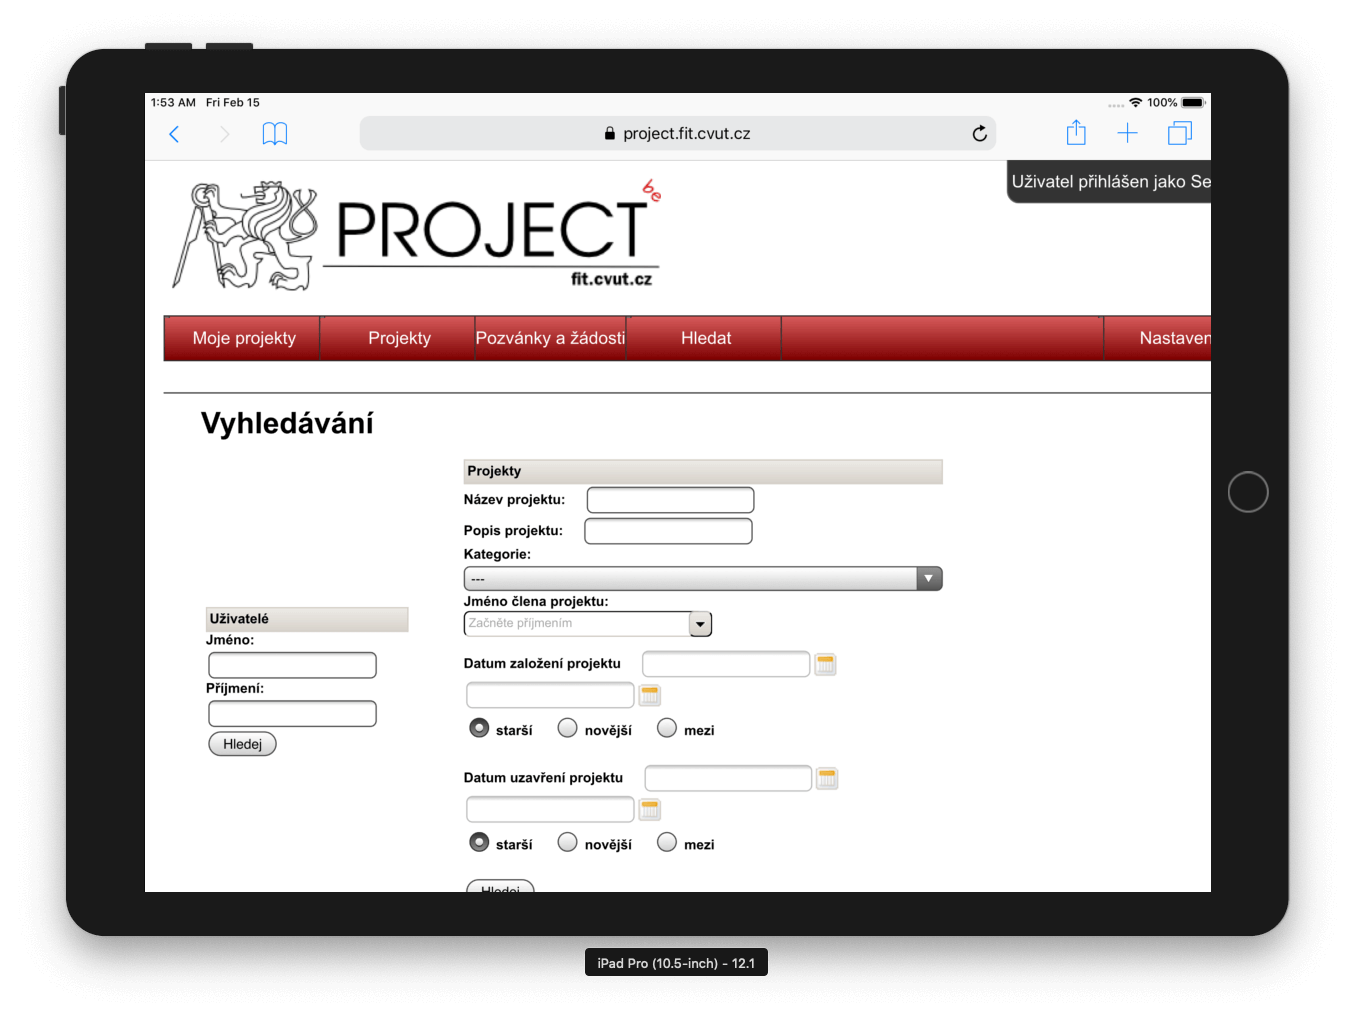
\includegraphics[width=1\textwidth]{images/analyza-swinpro.png}
   \caption{Ukázka vnitřní stránky portálu SwinPro}\label{pic:analyza-swinpro}
\end{fig:illustration}

SwinPro není uživatelsky pohodlnou aplikací, jeho webové rozhraní~\ref{pic:analyza-swinpro} není adaptováno pro současná zařízení. Při zobrazování stránek na menších obrazovkách se prvky rozhraní kriticky překrývají a není možné se dostat k překryté části. V dokumentaci nelze zobrazovat uvedené obrázky přímo v prohlížeči, jsou automatický staženy do zařízení.

\textbf{Pozitivní prvky}
\begin{ul}
   \item Každému projektu je umožněno automaticky přidávat individuální podpůrné nástroje.
\end{ul}

\textbf{Negativní prvky}
\begin{ul}
   \item Chaotické uživatelské rozhraní, které velice často neposkytuje přehlednou nabídku funkcionality.
   \item Neúplné a zastaralé informace napříč celým projektem vyvolávají pocit opuštěnosti portálu.
   \item Nelze zakládat studentské projekty, které by nebyly vedeny konkrétním vyučujícím.
\end{ul}


% --------------------------------------------------------------------------------------------------
% Moodle
% --------------------------------------------------------------------------------------------------


\section{Moodle FIT}

\textbf{Autor:} Centrum znalostního managementu FEL ČVUT\newline
\textbf{Analyzovaná verze:} Lassard 17\newline
\textbf{Datum analýzy:} 15.2.2019\newline
\textbf{URL:} \url{http://moodle.fit.cvut.cz/}

Moodle FIT~\cite{moodleFit} je webová aplikace založená na systému Moodle~\cite{moodle} a spravovaná Centrem znalostního managementu FEL ČVUT~\cite{czm}. Primárně plní roli poskytovatele základních informací o průběhu a hodnocení jednotlivých předmětů v konkrétních semestrech. V roce 2018 nahradila předchozí systém s podobnou funkcionalitou.

Kromě správy předmětů Moodle FIT rovněž dává možnost vytvářet online testy a definovat úkoly zvlášť pro každý předmět. Úkol je zobrazován v přehledu daného předmětu a definuje zadání a nejzazší termín odevzdání. Po splnění úkolu, což znamená nahrání jednoho či více souborů, se čeká na hodnocení se strany vedoucího. Po celou dobu nesplněného úkolu se na boční straně stránek zobrazuje upozornění se zbývajícím časem pro odevzdání. Získaný počet bodů za úkol je hned zobrazen v příslušné sekci přehledu předmětu. Může být doprovázen komentářem od vedoucího.


\begin{fig:illustration}
   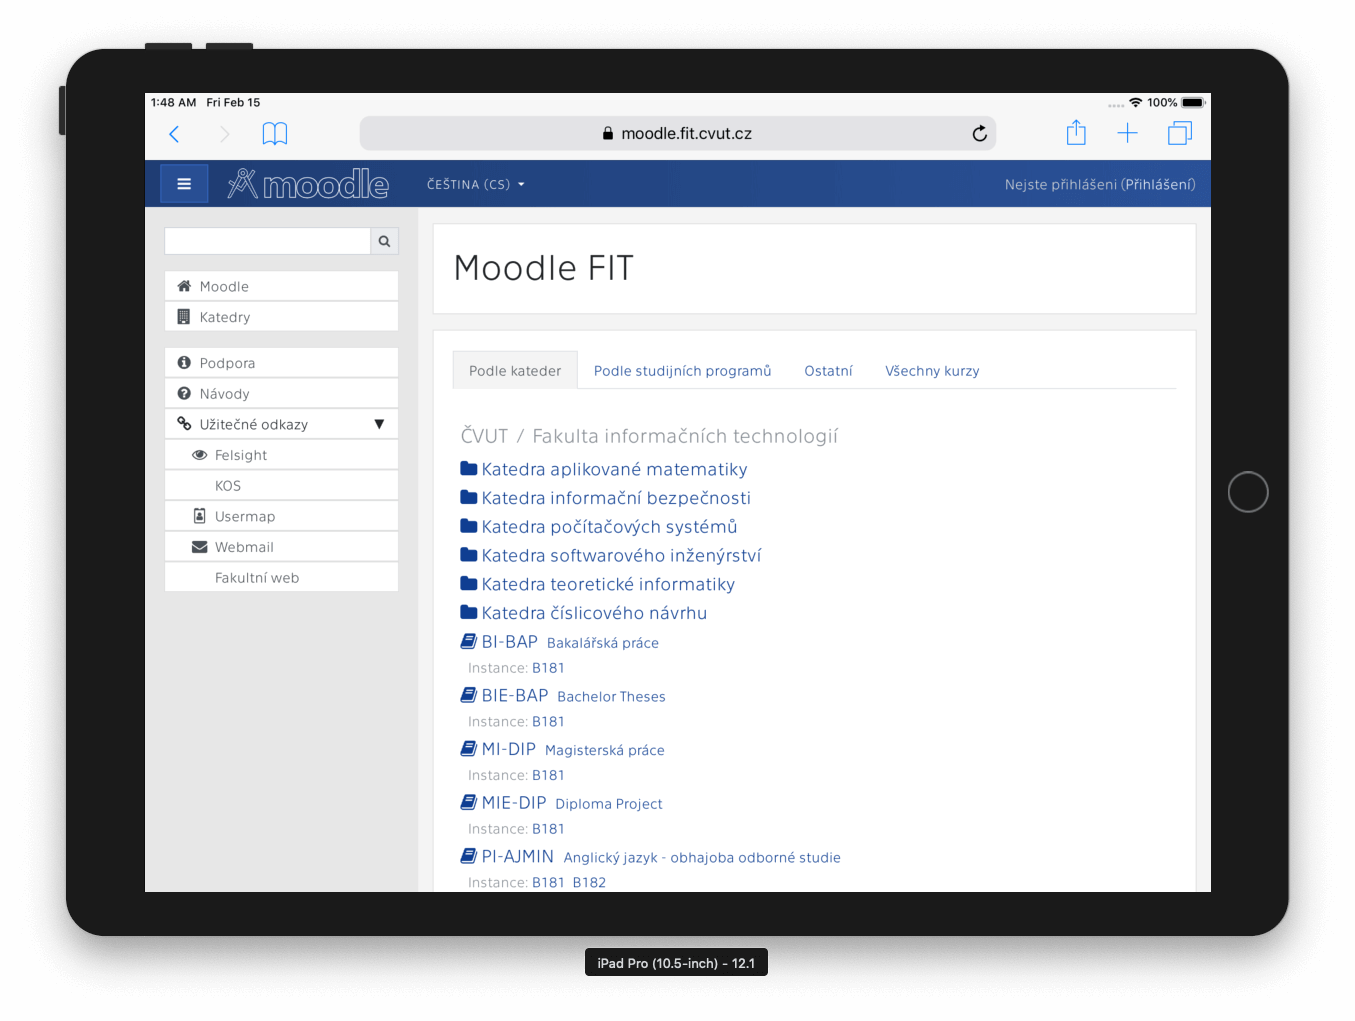
\includegraphics[width=1\textwidth]{images/analyza-moodle.png}
   \caption{Ukázka vnitřní stránky portálu Moodle FIT}\label{pic:analyza-moodle}
\end{fig:illustration}


Uživatelské rozhraní~\ref{pic:analyza-moodle} je adaptováno pro různé velikosti obrazovek, avšak realizovaná funkcionalita má často nepohodlné rozhraní. Vyhledávání na webu je velice omezené, není možné se dostat ke svým absolvovaným předmětům a tudíž i k odevzdaným úkolům.

\textbf{Pozitivní prvky}
\begin{ul}
   \item Zobrazování upozornění na nesplněné úkoly a zbývající čas.
   \item Komentáře vedoucího k odevzdanému úkolu.
\end{ul}

\textbf{Negativní prvky}
\begin{ul}
   \item Veškerá komunikace ohledně úkolu se provádí pouze prostřednictvím posílání souborů s následnou známkou a komentářem.
   \item Chybějící funkcionalita pro náhled a vyhledávání starších úkolů, jež se nachází v archivované podobě.
   \item Mnohdy neintuitivní uživatelské rozhraní.
\end{ul}


% --------------------------------------------------------------------------------------------------
% DBS
% --------------------------------------------------------------------------------------------------


\section{DBS portál}

\textbf{Autor:} kolektiv autorů (samostatně, bakalářské práce, diplomové práce)\newline
\textbf{Analyzovaná verze:} 4.21.0\newline
\textbf{Datum analýzy:} 14.2.2019\newline
\textbf{URL:} \url{https://dbs.fit.cvut.cz/}

Portál předmětu databázových systémů vyvíjený od roku 2014~\cite{dbsAuthors}. Ze studentského hlediska se jedná především o nástroj pro organizaci systematického odevzdávání průběžných částí semestrální práce, jež se píše během průchodu předmětem BI-DBS. Uplatnění nachází rovněž během semestrálního testu a závěrečné zkoušky, po zbytek času je však pro běžného studenta téměř zbytečný.

Organizace odevzdávání představuje systém dělení práce na tři navzájem závislé iterace, které definují jednotlivá kritéria pro jejich splnění. Každá následující iterace rozšiřuje či upravuje předchozí požadavky, mezi které se řadí datum odevzdání a plnění úkolů. Studenti zpracovávají práci do předem definovaných forem, například popis do textového pole, obrázek konceptuálního modelu do pole pro nahrávání souborů a další obdobná uživatelská rozhraní.

Po splnění kritérií jednotlivých iterací studenti mohou odevzdat aktuální stav práce jako celek pro hodnocení vedoucím práce. Některé části se hodnotí automaticky, něco však vyžaduje manuální kontrolu. Vedoucí práce rozhoduje o konečným počtu bodů za iteraci, jenž se zobrazuje studentovi na stránce celkového přehledu.

\begin{fig:illustration}
   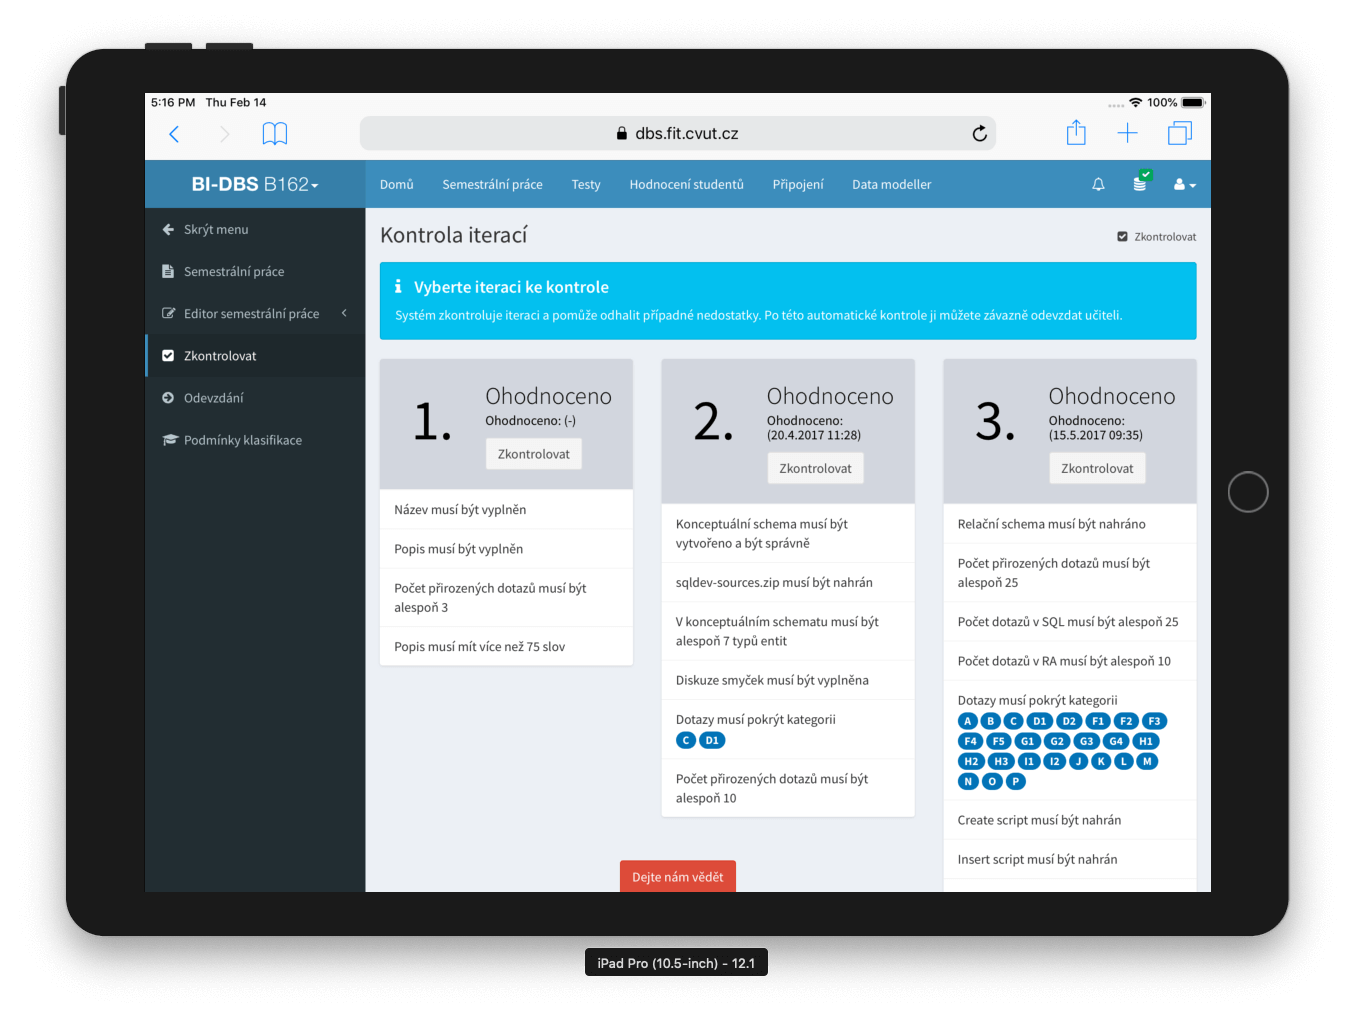
\includegraphics[width=1\textwidth]{images/analyza-dbs.png}
   \caption{Ukázka vnitřní stránky portálu DBS}\label{pic:analyza-dbs}
\end{fig:illustration}


Webové rozhraní~\ref{pic:analyza-dbs} je plně realizováno pro všechny běžné typy obrazovek a prohlížečů. Vychází z populární šablony ovládacího panelu AdminLTE~\cite{adminLTE}.

Daný webový portál je pozicován jako nástroj pro plnohodnotnou správu předmětu. Mimo správu semestrální práce nabývá možnosti data modelleru (modelování \gls{erd}), připojení ke školním či jiným databázím, přehledu anonymních výsledků studentů, vytváření průběžných semestrálních testů a závěrečné zkoušky s maximálně možnou automatizací kontroly výsledků. Veškerá tato funkcionalita není detailně analyzována z důvodu překročení rozsahu zájmu vytvářeného informačního systému.

\textbf{Pozitivní prvky}
\begin{ul}
   \item Existence stránky přehledu usnadňuje orientaci.
   \item Semestrální práce je dělena na iterace a následně na úkoly. Z hlediska studenta je to přehledné rozdělení práce.
   \item Některé úkoly je možné hodnotit automaticky.
\end{ul}

\textbf{Negativní prvky}
\begin{ul}
   \item Portál je zaměřen striktně na předmět databázových systémů. Není možné ho používat pro jakýkoliv jiný předmět bez kardinální změny implementace.
   \item Vedoucí práce nemá možnost okomentovat jednotlivé části práce. Realizovaná funkcionalita předpokládá pouze ohodnocení určitým počtem bodů.
\end{ul}


% --------------------------------------------------------------------------------------------------
% GitLab
% --------------------------------------------------------------------------------------------------

\clearpage
\section{GitLab}

\textbf{Autor:} GitLab Inc.\newline
\textbf{Analyzovaná verze:} Community Edition 11.3.14\newline
\textbf{Datum analýzy:} 15.2.2019\newline
\textbf{URL:} \url{https://gitlab.fit.cvut.cz/}

Fakultní nasazení aplikace GitLab poskytující v první řadě serverové úložiště pro Git repozitáře, systém sledování chyb, nastavení \gls{ci} a \gls{cd} a případné vytváření příručky typu wiki. Využívá se pro neveřejné studentské a fakultní projekty spravované \gls{vcs} Git.

Na základě GitLab je vytvořena webová služba Course Pages~\cite{courses}, která, stejně jako Moodle FIT, spravuje základní informace o předmětech. Mimo materiálů k jednotlivým předmětů se zde publikují zadání k semestrálním úkolům, jež studenti následně zpracovávají a odevzdávají buď fyzicky, nebo s pomocí jedné z komunikačních platforem.

\begin{fig:illustration}
   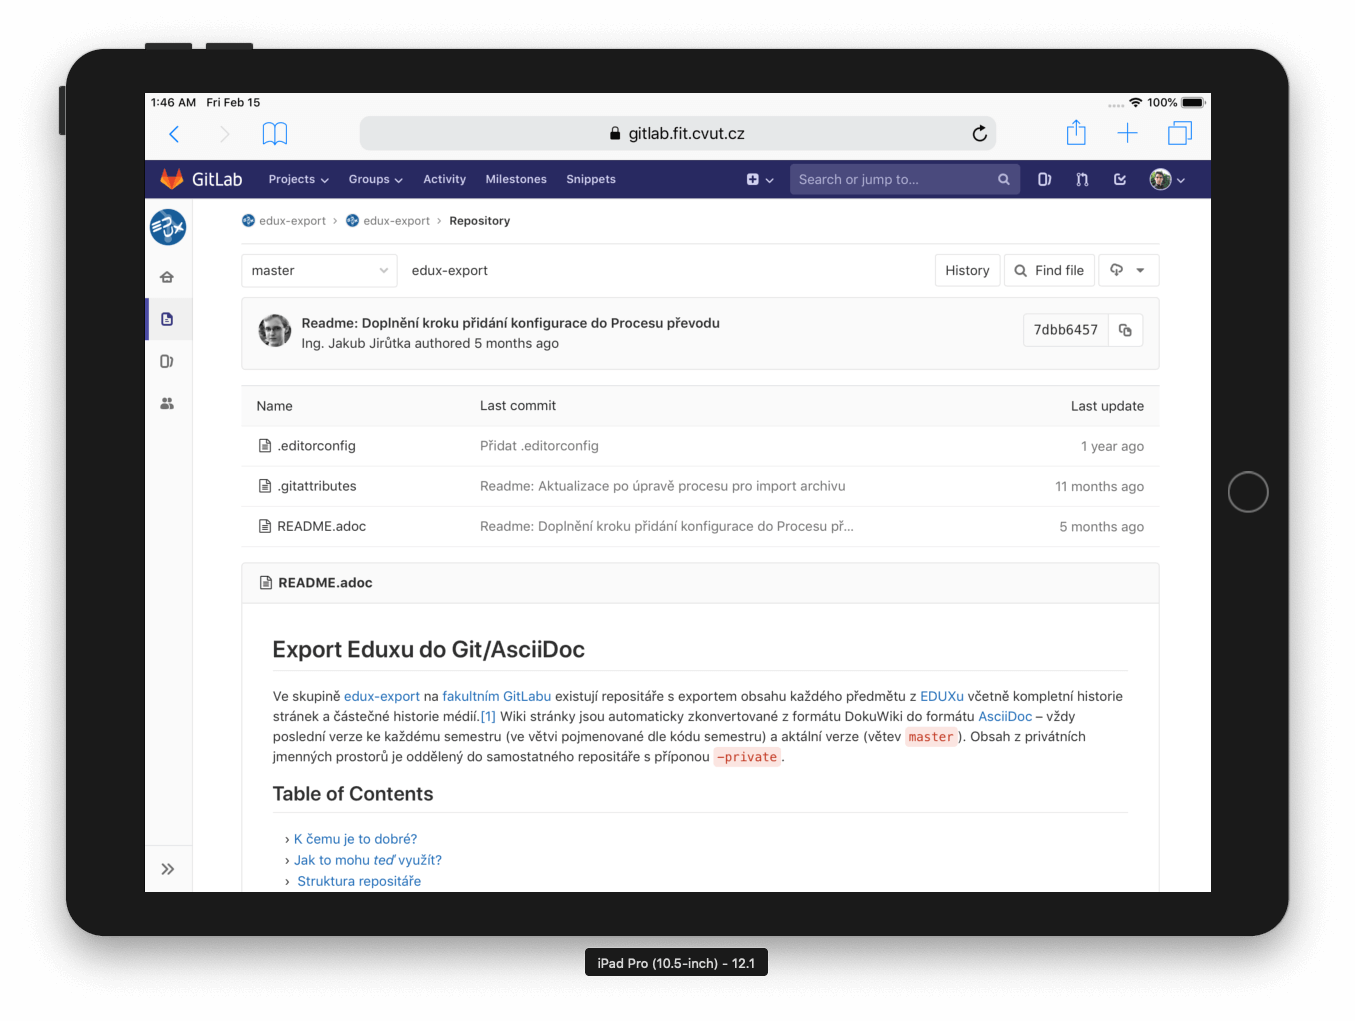
\includegraphics[width=1\textwidth]{images/analyza-gitlab.png}
   \caption{Ukázka vnitřní stránky GitLab}\label{pic:analyza-gitlab}
\end{fig:illustration}

GitLab je služba, jenž kolem sebe shromáždila obrovskou komunitu lidí~\cite{gitlabSource}. Uživatelské rozhraní~\ref{pic:analyza-gitlab} je udržováno se současnými standardy.

\textbf{Pozitivní prvky}
\begin{ul}
\tightlist
   \item Ohebný nástroj vyvíjený obrovskou komunitou mimo fakultu.
\end{ul}

\textbf{Negativní prvky}
\begin{ul}
   \item Pro používaní je nutné umět \gls{vcs} Git.
\end{ul}


% --------------------------------------------------------------------------------------------------
% Komunikační platformy
% --------------------------------------------------------------------------------------------------


\section{Komunikační platformy}

Pojmem komunikační platformy se v daném případě označuje skupina prostředků pro komunikaci, jež přímo není určena k udržování projektů, ale využívá se pro tento účel. Mezi takové paří Roundcube\footnote{Webmail}, Slack, Discord a další aplikace podobné struktury.

Roundcube se bere jako primární způsob komunikace mezi studenty a fakultou. Úkoly a semestrální práce zadané na cvičeních se většinou odevzdávají přes e-mail a výsledky se oznamují na jednom z dalších cvičení, či přímo do aplikace pro správu klasifikace daného předmětu.

\textbf{Pozitivní prvky}
\begin{ul}
   \item Intuitivní způsob komunikace, většinou není nutno se vyznat v základních možnostech používané služby.
\end{ul}

\textbf{Negativní prvky}
\begin{ul}
   \item V základní formě (bez rozšíření) pouze textová forma materiálů s případnými odkazy na vnější zdroje nebo soubory.
   \item Nepřehlednost předaných dat z hlediska verzování, komentování a hodnocení.
   \item Ztráta dat v dlouhodobém časovém úseku (automatické mazání zpráv, placená služba uchovávání většího množství dat, apod.).
\end{ul}


% --------------------------------------------------------------------------------------------------
% Fyzicka komunikace
% --------------------------------------------------------------------------------------------------


\section{Fyzická komunikace}

Klasická komunikace ověřená mnohaletými akademickými institucemi. V současné době se většinou obecně vyplácí pouze v případech, kdy výsledkem práce je jistý manuálně vytvořený objekt, jenž nelze převést do digitální podoby se zachováním jeho významu (například hardwarová součástka, fyzický model návrhu budovy).

Na \gls{fit} se tohoto způsobu odevzdávání využívá zejména v případech, kdy digitální podoba klade omezení na opravování práce. Jedná se například o opravu chyb ve výpočetních matematických příkladech, uvádění dodatečných vizualizací k určitým částem práce, apod.

\textbf{Pozitivní prvky}
\begin{ul}
   \item Kontrola odevzdané práce vedoucím projektu není závislá na jeho přístupu k internetu.
\end{ul}

\textbf{Negativní prvky}
\begin{ul}
   \item Nutnost se fyzicky dostavit na určité místo pro předání materiálů.
   \item Je nutné disponovat příslušnými zařízeními pro tisk.
   \item Doba od odevzdání po obdržení ohodnocené práce může být nepřiměřeně velká, pokud se nepoužívá jiný komunikační prostředek.
\end{ul}
